


\documentclass[10pt, handout]{beamer}
\setbeamertemplate{navigation symbols}{}
\usefonttheme{serif} 
\usepackage{amsmath}
\usepackage{amssymb}
\usepackage{graphicx}
\usepackage{cite}
\usepackage{color} 
\usepackage{setspace}
\usepackage{hyperref}

\newcommand{\xx}{{\bf{x}}}

\begin{document}
\title{Machine Learning I Lecture III:\\ Gaussian models}   
\author{Jakob H Macke\\ Max Planck Institute for Biological Cybernetics\\ Bernstein Center for Computational Neuroscience} 
\date{XY.XY.2012} 

\frame{\titlepage} 

%\frame{\frametitle{Today: Back to basics of probability theory}} 


\frame{\frametitle{Plan for today}\tableofcontents} 

\section{Wrap up: Continuous random variables}

\frame{\frametitle{Mean, variance, and conditioning on events are the same as the discrete case, just with sums replaced by integrals.}
\begin{itemize}
\item Mean: $E(X)= \int_x x  \cdot p(x) dx$\\
\item Variance: $\mbox{Var}(X)= E(X^2)- E(X)^2$
\item Example: Uniform, Exponential [on board]
\item \pause If $X$ has pdf $p(x)$, then $X | (X \in A)$ has pdf 
\begin{align}
p_{X|A}(x)=\frac{p(x)}{P(A)}=\frac{p(x)}{\int_{x \in A} p(x) dx}
\end{align}
\item \pause Only makes sense if $P(A)>0$~!
\item Examples: Uniform, Exponential [on board]
\end{itemize}
}



\frame{\frametitle{Bivariate continuous distributions: Marginalization, Conditioning and Independence}
\begin{itemize}
\item $p_{X,Y}(x,y)$, joint probablity density function of $X$ and $Y$
\item $\int_x \int_y p(x,y)dx dy=1$
\item \pause \alert{Marginal distribution:} $p(x)= \int_{-\infty}^\infty p(x,y) dy$
\item \pause \alert{Conditional distribution:} $p(x|y)= \frac{p(x,y)}{p(y)}$ 
\item Note: $P(Y=y)=0$! Formally, conditional probability in the continuous case can be derived using infinitesimal events.
\item \pause \alert{Independence:} $X$ and $Y$ are independent if $p_{X,Y}(x,y)=p_X(x)p_Y(y)$
\end{itemize}
}

\section{Gaussians}
\frame{\frametitle{The univariate Gaussian}
\begin{align}
t &\sim \mathcal{N}(\mu,\sigma^2)\\
p(t|\mu, \sigma^2)&=\frac{1}{\sqrt{2\pi\sigma^2}}\exp\left( -\frac{1}{2}\left(\frac{t-\mu}{\sigma} \right)^2\right)
\end{align}
\begin{itemize}
\item 
The Gaussian has \alert{mean} $\mu$ and \alert{variance} $\sigma^2$ and \alert{precision} $\beta=1/\sigma^2$
\item \pause Q: What are the \alert{mode} and the \alert{median} of the Gaussian?
\item \pause Maximum Likelihood estimation of $\mu$ and $\beta$: [on board]
\item \pause Q: How would you find the conjugate prior for the Gaussian?

\end{itemize}
}


\frame{\frametitle{A (very important) aside: Products of Gaussian pdfs are (unnormalized) Gaussians pdfs}
\begin{itemize}
\item Suppose $p_1(x)=\mathcal{N}(x,\mu_1, 1/\beta_1)$ and $ p_2(x)=\mathcal{N}(x,\mu_2, 1/1\beta_2)$, then  
\pause \begin{align}
p_1(x) p_2(x) &\propto \mathcal{N}(x, \mu, 1/\beta)\\
\beta&=\beta_1+\beta_2\\
\mu&=\frac{1}{\beta}(\beta_1 \mu_1 +  \beta_2 \mu_2)
\end{align}

\pause 
In general:
\begin{align}
p_1(x) p_2(x) ... p_n(x) &\propto \mathcal{N}(x, \mu, 1/\beta)\\
\beta&=\sum_n \beta_n\\
\mu&=\frac{1}{\beta} \sum_n \mu_n \beta_n
\end{align}

\pause 
This is also true for multivariate Gaussians!

\end{itemize}
}


\section{Bayesian inference for Gaussians}

\frame{\frametitle{Bayesian Inference for the Gaussian}
\begin{itemize}
\item Suppose we are given data $D=\{x_1, \ldots, x_N\}$. 
\item We assume that the data is Gaussian-distribution with known variance $\sigma^2$ and unknown mean $\mu$.
\item Our prior for $\mu$ is Gaussian: $\mu \sim \mathcal{N}(\mu_o, \sigma^2_o)$
\item Posterior distribution over $\mu$ given the data: [on board] 
\end{itemize}
~
\pause
{\centering
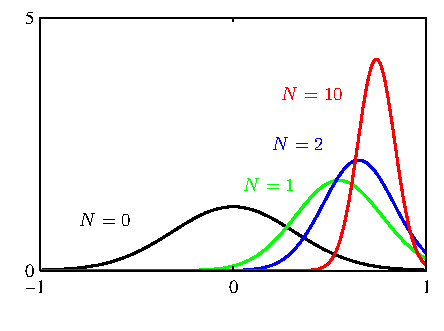
\includegraphics[width=.58\textwidth]{Figure212.pdf}
\\\vspace{-.5cm}}
{\tiny[Bishop PRML Figure 2.12]}

\pause Behaviour for large $N$: [on board]
}

\frame[shrink=0]{\frametitle{What if the variance is not given?}
\begin{itemize}
\item For simplicity, assume mean to be known.
\item More convenient to work with precision $\lambda=1/\sigma^2$.
\item Conjugate prior: Gamma distribution $\mbox{Gam}(\lambda|a,b)$
\begin{align}
p(\lambda|a, b)=\frac{1}{\Gamma(a)}b^a \lambda^{a-1} exp(-b\lambda)
\end{align}
\item Posterior is $\mbox{Gam}(\lambda|a_N,b_B)$
\begin{align}
a_N &= a + \frac{N}{2}\\
b_N &= b + \frac{1}{2} \sum_{n=1}^N (x_n -\mu)^2
\end{align}
\pause
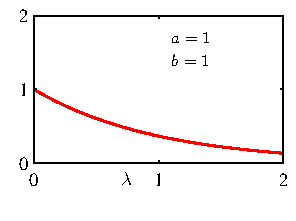
\includegraphics[width=.38\textwidth]{Figure213b.pdf}
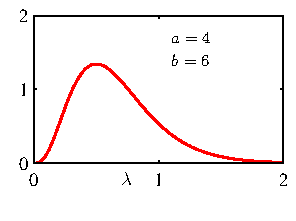
\includegraphics[width=.38\textwidth]{Figure213c.pdf} \\\tiny[Bishop PRML Page 100]

\end{itemize}
}

\frame[shrink=0]{\frametitle{What if both the mean and the variance are unknown?}
\begin{itemize}
\item Conjugate prior: Gaussian-Gamma distribution
\begin{align}
p(\mu,\lambda) & = \mathcal{N}\left(\mu |\mu_o (\beta\lambda)^{-1}\right) \mbox{Gam}(\lambda|a,b)
\end{align}s
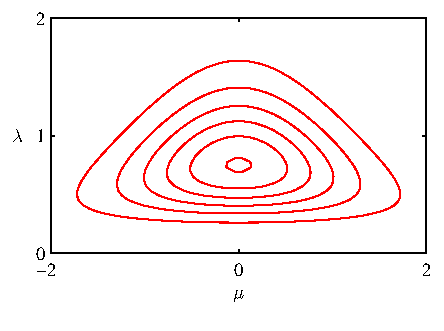
\includegraphics[width=.68\textwidth]{Figure214.pdf} \\\tiny[Bishop PRML Page 102]
\end{itemize}
}




 
\end{document}



